\documentclass{article}
\usepackage[top=2.4cm, bottom=2.4cm, left=1.8cm,right=1.8cm]{geometry}
\usepackage{amsmath} 
\usepackage{amssymb} 
\usepackage[retainorgcmds]{IEEEtrantools}
\usepackage[titles]{tocloft}
\usepackage{makeidx} 
\usepackage{graphicx} 
\usepackage{color}
\usepackage{listings}
\usepackage{booktabs}
\usepackage{float}
\restylefloat{table}
\usepackage[refpage,intoc,norefeq]{nomencl} 
\usepackage{lipsum}
\usepackage[toc,page]{appendix}
\usepackage[round,sort&compress,authoryear,numbers]{natbib}  
\usepackage[numbib]{tocbibind}
\usepackage[pdftex,backref=page]{hyperref}
\usepackage{hyperref}
%\usepackage{minted}
\usepackage{xcolor}
\usepackage{courier}
\usepackage{longtable}
\usepackage{lmodern}

\usepackage{pgfplots}
\usepgfplotslibrary{external}
\pgfplotsset{width=7cm,compat=1.11}


\tikzexternalize[prefix=figures/]% activate with a name prefix

\begin{document}
\begin{figure}
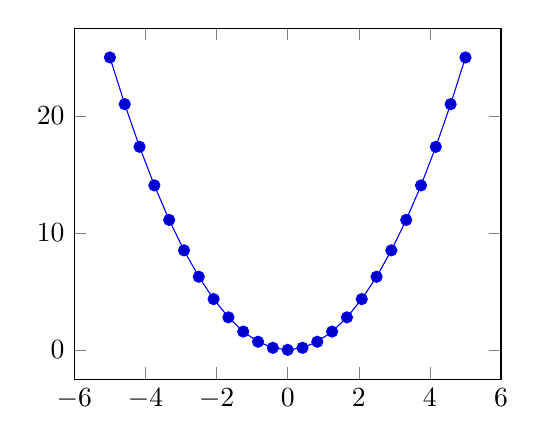
\begin{tikzpicture}
\begin{axis}
\addplot {x^2};
\end{axis}
\end{tikzpicture}
\caption{Our first external graphics example}
\end{figure}


\begin{figure}
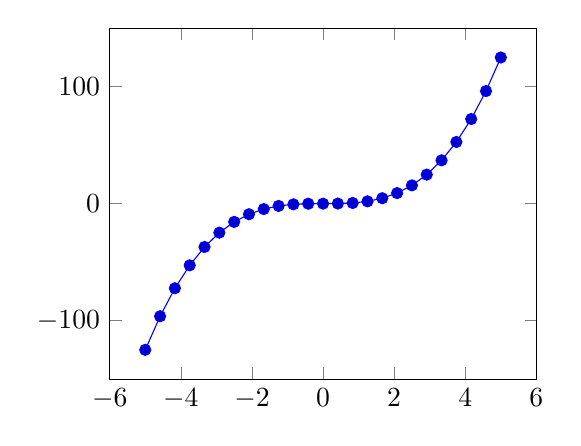
\begin{tikzpicture}
\begin{axis}
\addplot {x^3};
\end{axis}
\end{tikzpicture}
\caption{A second graphics}
\end{figure}




\tikzsetnextfilename{3Dplot}
\begin{figure}
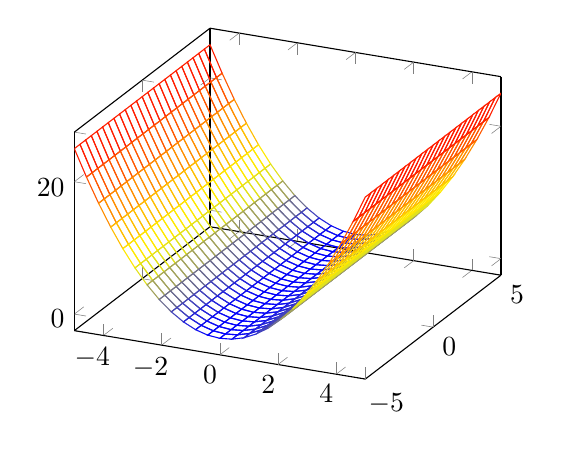
\begin{tikzpicture}
\begin{axis}
\addplot3[mesh] {x^2};
\end{axis}
\end{tikzpicture}
\caption{Our third external graphics example}
\end{figure}


\tikzsetnextfilename{Surfaceplot}
\begin{figure}
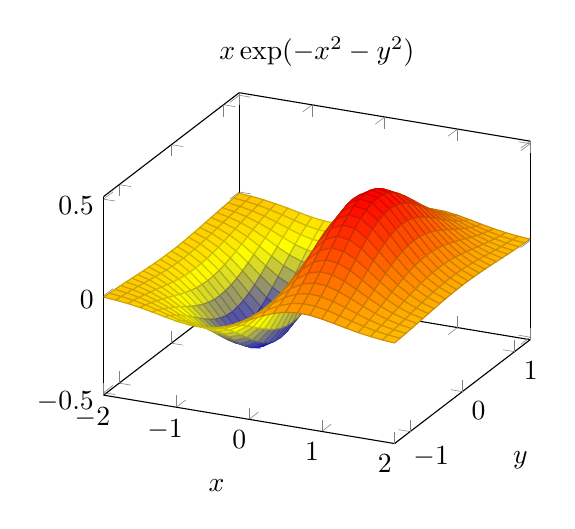
\begin{tikzpicture}
\begin{axis}[
title={$x \exp(-x^2-y^2)$},
xlabel=$x$, ylabel=$y$
]
\addplot3[
surf,
domain=-2:2,
domain y=-1.3:1.3,
]
{exp(-x^2-y^2)*x};
\end{axis}
\end{tikzpicture}
\caption{Our fourth external graphics example}
\end{figure}


\tikzsetnextfilename{normaldist}
\begin{figure}
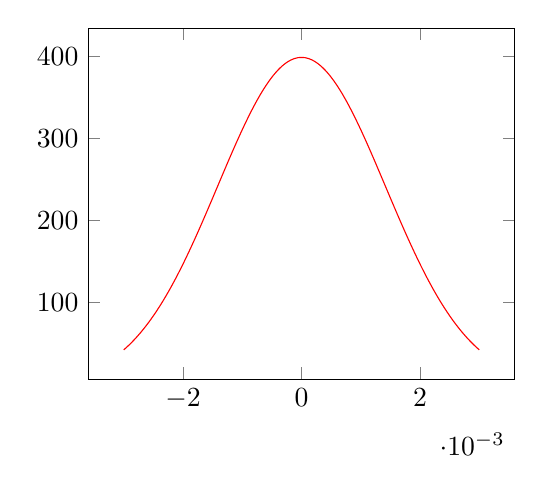
\begin{tikzpicture}
\begin{axis}[
]
% density of Normal distribution:
\addplot[
red,
domain=-3e-3:3e-3,
samples=201,
]
{exp(-x^2 / (2e-3^2)) / (1e-3 * sqrt(2*pi))};
\end{axis}
\end{tikzpicture}
\caption{Our fifth external graphics example}
\end{figure}



\end{document}
